\documentclass[a4paper, parskip=true, firsthead=false, fromemail=true, foldmarks=false]{scrlttr2}
\usepackage[utf8]{inputenc}

\setkomavar{fromemail}{mathieu.leocmach@univ-lyon1.fr}
\setkomavar{signature}{Hassan Srour, Martien Duvall Deffo Ayagou, Thi Thanh-Tam Nguyen, Nicolas Taberlet, S\'{e}bastien Manneville, Chantal Andraud, Cyrille Monnereau, and Mathieu Leocmach}


\usepackage{amsmath}
\usepackage{amsfonts}
\usepackage{amssymb}
\usepackage{graphicx}
\usepackage[british]{babel}

\usepackage{kpfonts}
\usepackage{tabu}
\usepackage{wrapfig}
\setlength{\columnsep}{0.05\textwidth}
\usepackage{ifthen}
\usepackage{hyperref}
\usepackage{enumitem}
\setlist{nosep}

%\usepackage{tikz}
%\definecolor{ilmcolor}{RGB}{177,37,159}
%\definecolor{ilmorange}{RGB}{255,116,40}
%\usetikzlibrary{arrows,shapes,backgrounds, calc, positioning, topaths,chains, intersections, decorations.markings, decorations.text, shapes.geometric, matrix,patterns,mindmap,fit}

\newcommand{\journal}{Soft Matter}

\begin{document}
\begin{letter}{From:\\
Mathieu Leocmach,\\
Univ Lyon,\\ 
Universit\'e Claude Bernard Lyon~1, CNRS,\\
Institut Lumi\`ere Mati\`ere,\\
F-69622, VILLEURBANNE,\\
France\\
\texttt{mathieu.leocmach@univ-lyon1.fr}
}
\opening{\bf Dear Editor,}

\begin{wrapfigure}[16]{r}[0pt]{0.25\textwidth}
\hfill
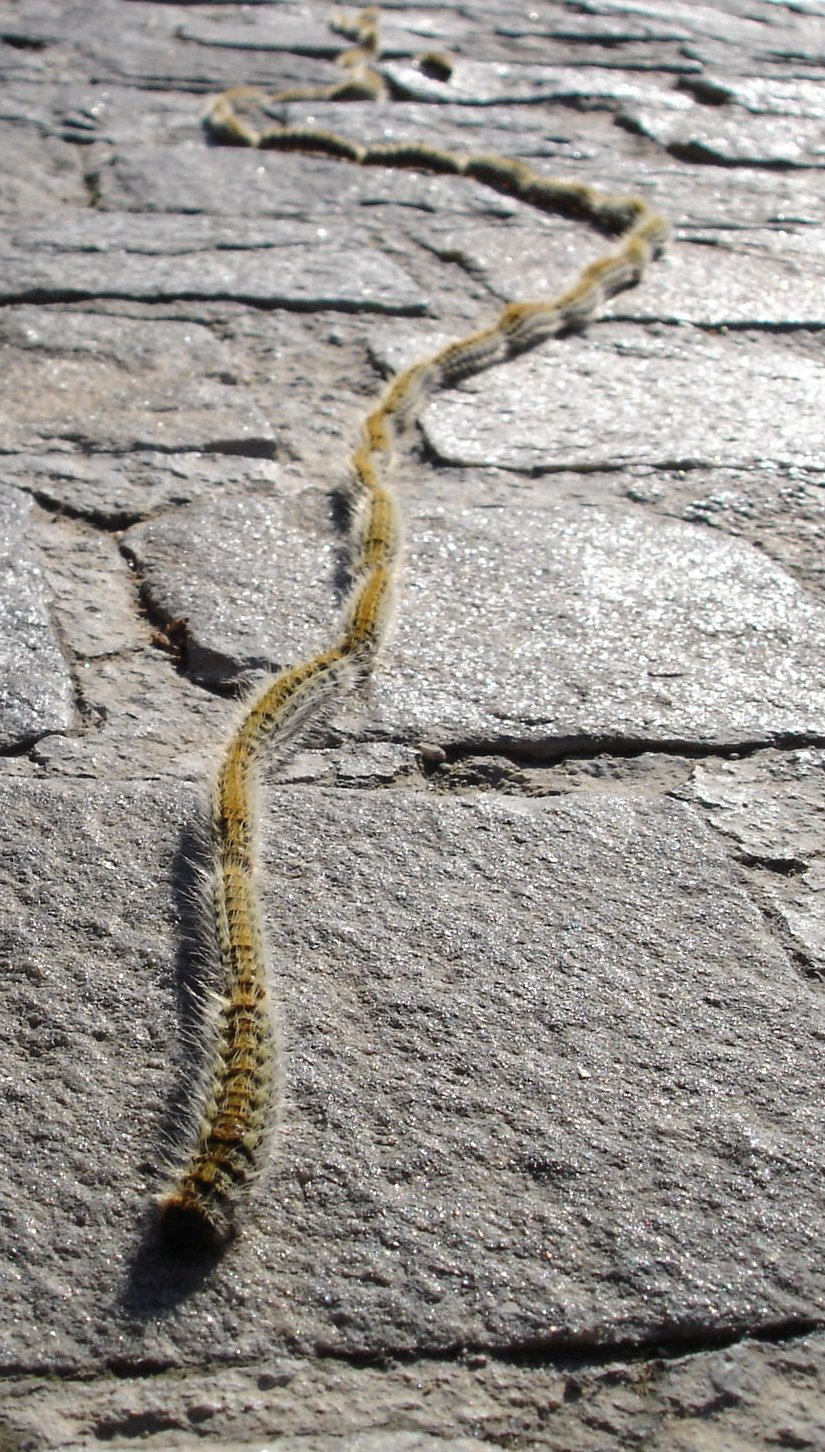
\includegraphics[width=\linewidth]{presentation/Thaumetopea_pityocampa_01.jpg}

\raggedright
Pine processionary caterpillars
\end{wrapfigure}

Please find enclosed our manuscript, entitled \textsc{Ion pairing controls rheological properties of ``processionary'' polyelectrolyte hydrogels}, which we are submitting for publication as an article to \journal.

Polymer-based hydrogels have promising biomedical applications, eg. as a soft scaffold for cellular growth. To be used in vivo, solid pieces of gel have to be implanted surgically. By contrast a physical gel with a yield stress rheology would allow a a much less traumatic delivery via injection: solid in the syringe, the gel could flow through the needle and reform as a solid once in the body. In the present work we design and study such a polymeric physical gel.

The system we investigate is made of short (70 units) linear polymer chains. In aqueous solution, a single extremity (the `head') is charged negatively whereas the repeated unit of the `body' carries a positive charge. We demonstrate that these chains self assemble into long processions (up to 800 chains) due to electrostatic interactions. %These processions are entangled or cross-linked on the scale of the screening length. 
The resulting physical hydrogel behaves as a yield stress fluid. In this article we build a microscopic understanding of the chemical physics involved in this gel that allows us engineer its rheological properties.

We have demonstrated previously [\href{ https://doi.org/10.1002/marc.201400478}{Srour et. al, Macromol Rapid Commun. 2015.}] how to obtain well-controlled anion-terminated poly(cationic) polymer via atom transfer radical polymerisation and post-functionalisation. Here we harness the power of this post-functionalisation approach to systematically alter the repeated unit. From a common scaffold we generate a family of such polyelectrolytes where the cationic moieties can be either all aromatic (imidazolium) or all aliphatic (pyrrolidinium), with counterions ranging from fluoride to iodide along the Hofmeister series. We show that the resulting difference in counterion condensation alters the rheological properties of the resulting hydrogel over three orders of magnitudes.

From these experimental results, we develop the ``processionary'' model briefly exposed above. This model builds on the scaling theory of polyelectrolytes gels and allows us to quantify microscopic observables (e.g. the amount of counterion condensation, head-to-body bonding energy) from standard macroscopic rheology procedures (oscillatory strain amplitude sweep). Conversely this model exposes all the relevant parameters we can tune to design physical hydrogels with desired rheological properties.


Our findings are at the interface between polymer chemistry and rheology, bridged by an understanding of the underlying physics, with possible biomedical applications.

We hope that you will find that the paper is interesting enough to be published in \journal. 

We suggest the following scientists as possible reviewers, by alphabetical order:
\begin{enumerate} \setlength\itemsep{0em}
\item Andrey V. Dobrynin, University of Connecticut, 
avd@ims.uconn.edu
\item Elie Raphaël, UMR CNRS Gulliver 7083, ESPCI, elie.raphael@espci.fr
\item Michael Rubinstein, University of North Carolina, mr@unc.edu
\item Annette M. Schmidt, University of Cologne, annette.schmidt@uni-koeln.de
\item Nadine Schwierz, University of California, Berkeley, nschwierz@berkeley.edu
\end{enumerate}


Warm thanks to you for your kind attention and cooperation. 


\closing{\bf Sincerely yours,} 

\end{letter} 
\end{document}